\chapter{Conclusion}
\label{chap:Conclusion}
In this chapter I will sum up what have been made. I will compare the resulting
product with the requirements of Chapter~\ref{chap:Domain analysis}. After this
I will conclude on the product, looking at advantages and disadvantages in the
way I have decided to make it.
In the end I will have a discussion of what future work should and could be made
for the system to be ready to be set into production. Ending with a statement
from IT minds about the project.

\section{Summery}
IT minds is a consultant company consisting of mostly student developers who has
been taught Java and maybe C\#. For the developers to have anything to do the
company has sales teams who is responsible of getting tasks for the developers.
In order for them to be able to keep track of the people they talk to, and the
opportunities they get they use a customer relations management system, or CRM
for short. 

The current CRMs are not capable of doing what IT minds require entirely, and
therefore I have gotten the job of making a prototype of an alternative. An
introduction to the system in presented in Chapter~\ref{chap:Introduction}.

The Idea is that it should be possible to get an overview of how it is going in
the system, both in regard to how much is being sold, and how much is supposed
to be sold. This should be filterable, so that one can decide only to see for
one office instead on the entirety of IT minds, even though that should also be
possible. 

Another important feature is the ability to define categories, and
values in the system as an admin, since this allows for setting the system
up exactly as is desired, instead of having to force some predetermined setup by
the developer on the sales team.

In Chapter~\ref{chap:Domain analysis} I discuss what exactly the system is
supposed to be capable of, such as the number of user levels, and the
visualization.

In this chapter I also set up the functional and nonfunctional requirements of
the system, and combine them with use cases which are also described here. This
Is also where I describe the domain model of the system, which later on is used
to find the resources the system should present, as well as help with designing
the ER diagram for the database. At the end of the chapter I present a suggestion
to how some of the views that is described by use cases could look.

Based on the requirements I discussed the possible technologies in
Chapter~\ref{chap:Technology}. Since IT minds had limited requirements to the
technologies I was fairly free to go with what I felt was fitting, which is why
I have compared a couple different ones in that chapter. A thing that I did keep
in mind is the use of C\# in IT minds projects, which leads to most IT minds
developers knowing that language. This is a concern since it would probably be
a developer from IT minds who would end up extending and supporting my solution
in the future.

I looked at both web services and static serving as possible technologies,
concluding a web service would be better, as it does not limit the front-end,
allowing for an app for phones or desktop in the future if that is deemed suited.

After I settled for a web service, I had to decide which type. The two I
compared was REST, and SOAP.\ Where I ended up with REST, as it is potentially
easier to interpret the result in JavaScript, which is what I have made the
front-end part in. For the data I send  I went with JSON, for that exact reason,
and because it is easy to read, and therefore validate when building the service.

For the database I compared a few types, and settled for a relational one named
MsSQL, with the entity framework for access, mostly because it has good support
in the .NET environment.

The front-end was not discussed as in depth, as it is more a suggested
implementation of how one might look, and as I don't have any proper knowledge
of building a user friendly interface I cannot claim that what I have build
follows the rules that is required for that. 

The reason I still build a front-end was two fold however, as it allowed me to
think in a more user near way when developing the resource paths, and it allowed
me to integration test a bit easier. It is also easier to show others what I
have made if it has a user interface, instead of just being data dumped out by a server.

In Chapter~\ref{chap:Design} I discuss the design of the system. First I create
the design of the database, described with an ER diagram. The database is only
in 2NF.\ The reason I have not made it 3NF is that this would make it hard to
work with the entities, where it has any influence. The actual issue is that a
company has an address, which could be separated out into a separate table, but
this is also true for the country, and an address should have a country
associated with it then, which would mean that every time a new company is added
I would have to check if a country of the same name exists, and I cannot know if
the user just spelled the name wrong.

For the structure of the system I have followed the onion model separating the
system out in layers, always only referencing deeper, and never up.

In this chapter I also created some sequence diagrams describing two use cases
all the way from client to database and back. I also have a short description of
some class diagrams of the system.

Near the end of the chapter I describe some of the patterns I use in the
development, such as dependency injection, and the repository pattern.

In the end the implementation has been described in
Chapter~\ref{chap:Implementation}. Here I discuss my use of the entity
framework, and how I even though it is already using the repository pattern, and
unit of work pattern, I wrap it in order for me not to be as dependent on the
ORM itself in the controllers.

In the implementation I also discuss how I handle cascade delete, as there are
some issues with circular paths if it is automated in some cases.

For fails caused by something that the repositories need, such as not finding a
resource, or duplicate where it should be unique I throw exceptions which is caught by a filter
and converted into the proper HTTP response.

I also discuss how I get the data from the database and format it in a way so
that it can be plotted in a graph, with a few code examples.

The last part of the Chapter~\ref{chap:Implementation} is about how I have
tested the system, and some of the advantages the different testing methods
have. Here I describe the idea behind the testing, including how the unit
testing has been done, and what frameworks I used. I also explain how it is
easier to test isolated parts of the code in the unit tests because of the
dependency injection. Another thing I go over in this part is the integration 
testing, even though I have not made too many automated integration tests, but
rather taken advantage of the web application to test the flow of the data.

\section{Conclusion}
The development of the prototype has fulfilled the vision, in that it is
possible to ask the service for data to be graphed. The data is extracted by
calling an HTTP route on the server, and an example web application has been
made to illustrate a possible way to handle the data to make graphs.

Because the web service is made as an API, there is good extensibility in regards
to front-ends, so it will be possible to create a web service, phone or desktop
application without changing the back-end.

For future development such as the features suggested in
Section~\ref{sec:future_work}, and other features required for the service to
work competitively compared to other CRMs, the server is created in such a way
that it is not necessarily required to deal with the existing code, depending on
what is to be implemented.

The front-end that has been developed will require at least someone with
experience in user experience design to take a look, as it has only been
developed with the intention of giving an idea of how the system could look.

The cooperation with IT minds has given a good guideline in regards to what the
system should be able to do, and the meetings with Kristian has been really
helpful in keeping me from running out on a tangent in the development, and to
give ideas on what should be developed next for the system to be usable by him
and the rest of the sales team.

Overall the service and web application IT minds have received works well, and
fulfills the requirements. It supports extension without too much trouble, and
can easily support another front-end when that is deemed necessary.

\section{Future work}
\label{sec:future_work}
Since the product I have created only is a prototype, it is not currently in a
state where IT minds would be able to take it into use, but requires some
adjustments and a few features before that would be possible.

One thing that should be looked at would be the \textbf{user experience}, as for a system
like this to succeed a user and a designer would have to sit down and spend
some time looking at workflows and from that develop a proper interface that
suites the work flows of such a system.

In IT minds we use Google as our email host, and as such have our Google
accounts associated with a lot of web applications, therefore it would make sense to
allow us to use Google for the CRM as well. The way I have developed the user
authentication it would be possible to include Google accounts and single
\textbf{sign-on}. It would also be possible to use Facebook, twitter, or Microsoft accounts if that
is something that makes sense. The extension would not require too much work,
and it would not necessarily break the current login flow, but rather extend it
with the possibility of alternatives.

Another feature that could be useful in the future would be the integration of
calendars, so that a user can go in and see in a \textbf{calendar view} the assignments
they have. This would allow the users to get a better overview of what they have
to do and when. The feature is mostly supported in the back-end currently, so
the only real change in the back-end would be the ability to filter an activity
based on the date and possibly time it is happening.

An extension to the calendar view could be the full integration of \textbf{external
calendars}. An example of such an integration could be Google calendar, which is
used a lot in IT minds, as it is part of our mailing system as described
earlier. For proper usability it would probably have to support several
different calendar types and be configurable so that a user would be able to
choose not to get every type in to their calendar. The customization could be
based on activity categories, so the user could choose if they want all, some,
or none of the categories added to their calendar.

In relation to that it could be useful to be able to \textbf{automatically create
activities} by inviting the system into an event. This could as an example work
so that if Kristian wanted to create an activity with me he would create a
Google calendar event and invite me. In IT minds he would usually also add the
meeting room, to book it so others can see that it is not available at the given
time. In a similar fashion he could then add the system as a participant, and
when it receives an invitation it would create an activity for Kristian and me.
In the case no person in the system has my email it would have to add a new
person and probably inform Kristian that he should update the information on
that person. For the company it could be left blank, or the system could try to
interpret it based on the host name of the email address.

Another thing that would possibly be good for the system would  be to \textbf{improve
the filter} that a user could apply when looking at the overviews, allowing them
to filter only on people from eg.\ a specific company. This would require some
adjustments in what is received from the front-end, but since the database is
build up in a relational way the search itself is not hard, but figuring out how
to allow a user to search for any given number of parameters at once may be a
challenge, although not impossible.

A thing that would require some improvements for it to work satisfyingly is the
\textbf{searching feature}. Right now this feature only matches for almost exact words,
meaning misspellings are not accepted, and the only acceptable differences in
the words are spaces and dashes, as i remove those from the search term and the
target word. I also make sure that there are no issues with upper or lower case
letters, but it still means that the term would have to be consisting of only
letters in the desired word, in the correct order.

When I make the production graph data setup I figure out how to split the
earnings based on months, which for a better effect should be based on number of
days in a month, ideally \textbf{workdays per month}. The result of this would be that if
1.000.000 kr.\ was set from 2016--02--09 to 2016--03--11 the amount for February
would be 640.000 kr.\ and 360.000 kr.\ for March as there are 16 work days from
the 9th of February to the end of the month and 9 from the start of March to the
16th. This would also help with calculating the money the person who made the
sale should get for each month, and give an even better idea of how the
developer resources are allocated.

\section{IT minds statement}
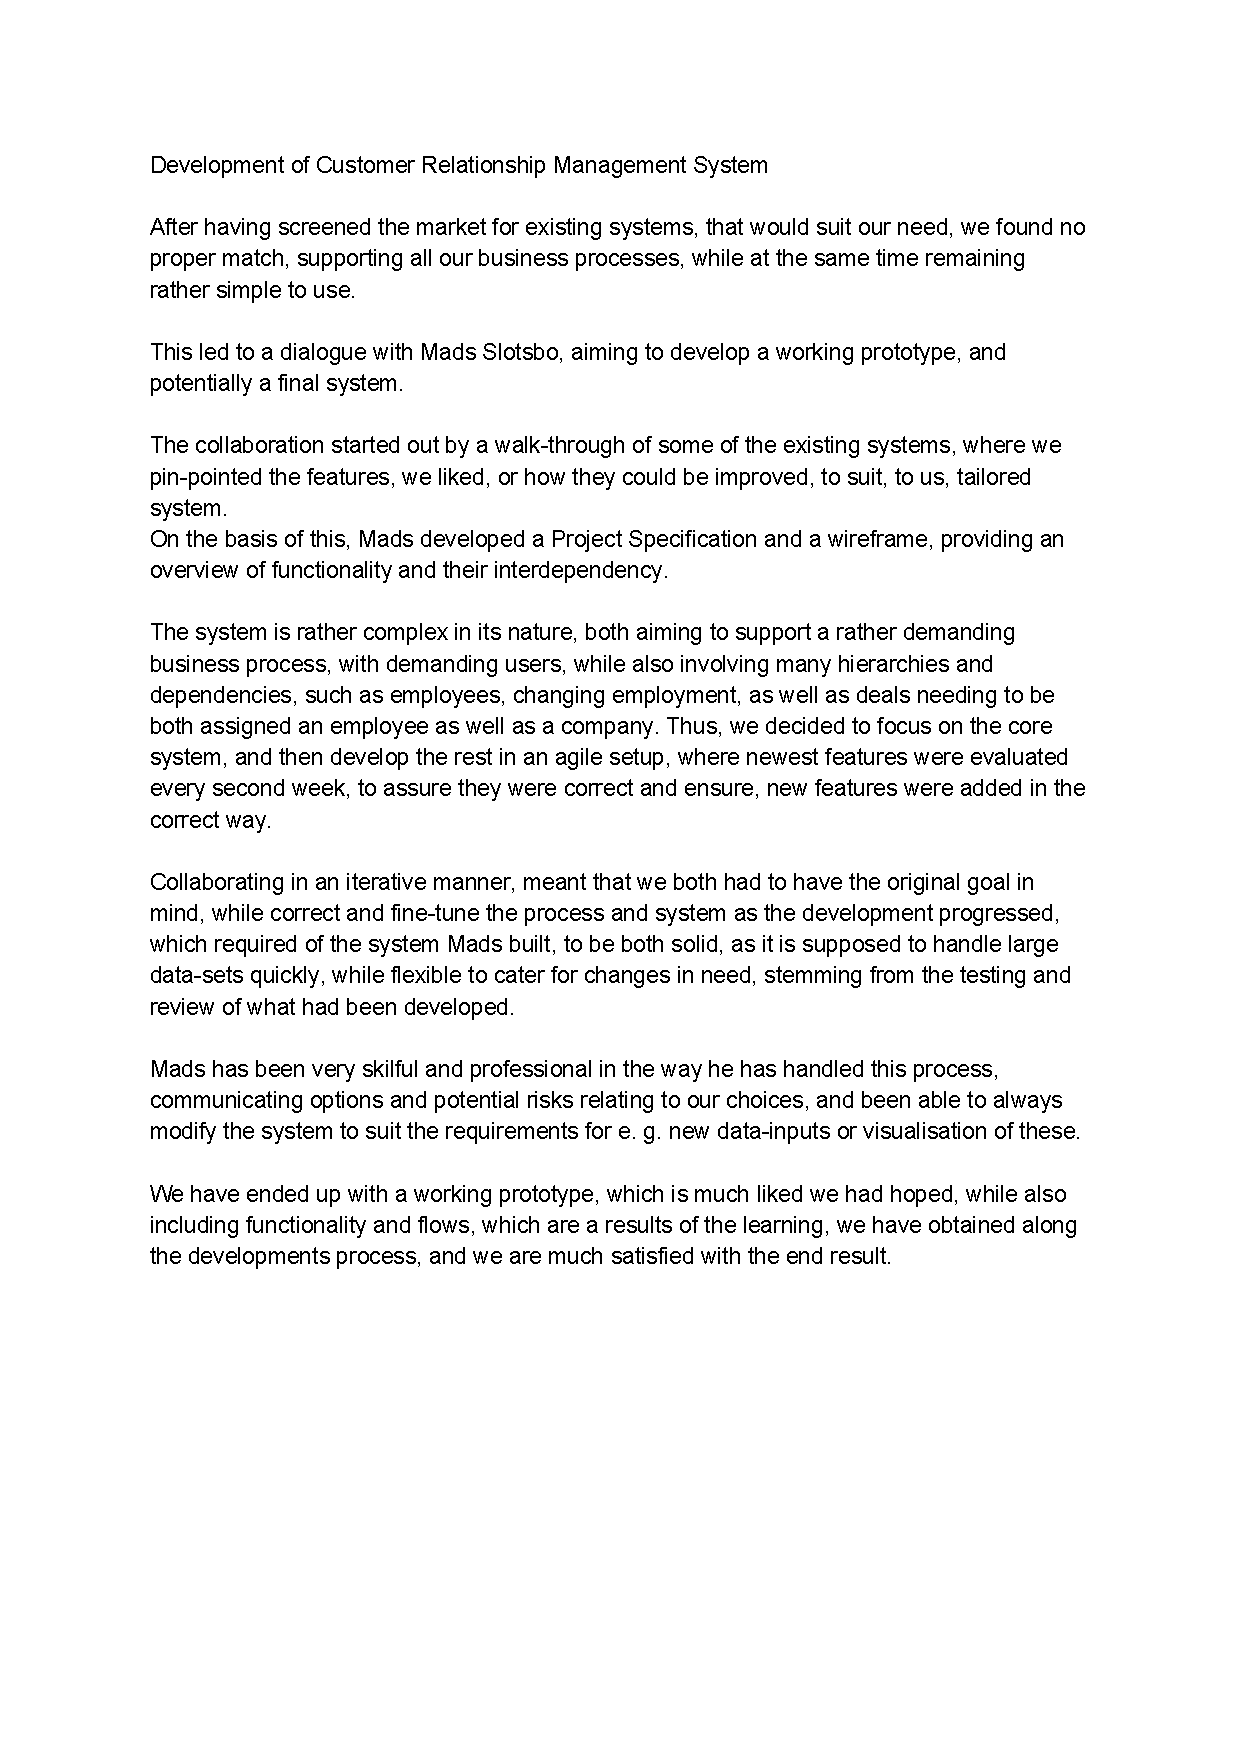
\includegraphics[width=1.2\textwidth]{201604-MadsSlotsboCRM}